\PassOptionsToPackage{unicode=true}{hyperref} % options for packages loaded elsewhere
\PassOptionsToPackage{hyphens}{url}
%
\documentclass[]{article}
\usepackage{lmodern}
\usepackage{amssymb,amsmath}
\usepackage{ifxetex,ifluatex}
\usepackage{fixltx2e} % provides \textsubscript
\ifnum 0\ifxetex 1\fi\ifluatex 1\fi=0 % if pdftex
  \usepackage[T1]{fontenc}
  \usepackage[utf8]{inputenc}
  \usepackage{textcomp} % provides euro and other symbols
\else % if luatex or xelatex
  \usepackage{unicode-math}
  \defaultfontfeatures{Ligatures=TeX,Scale=MatchLowercase}
\fi
% use upquote if available, for straight quotes in verbatim environments
\IfFileExists{upquote.sty}{\usepackage{upquote}}{}
% use microtype if available
\IfFileExists{microtype.sty}{%
\usepackage[]{microtype}
\UseMicrotypeSet[protrusion]{basicmath} % disable protrusion for tt fonts
}{}
\IfFileExists{parskip.sty}{%
\usepackage{parskip}
}{% else
\setlength{\parindent}{0pt}
\setlength{\parskip}{6pt plus 2pt minus 1pt}
}
\usepackage{hyperref}
\hypersetup{
            pdftitle={Dataset Analysis and CNN Models Optimization for Plant Disease Classification},
            pdfauthor={Claudio Moroni \textbar{} Davide Orsenigo \textbar{} Pietro Monticone},
            pdfborder={0 0 0},
            breaklinks=true}
\urlstyle{same}  % don't use monospace font for urls
\usepackage[margin=1in]{geometry}
\usepackage{graphicx,grffile}
\makeatletter
\def\maxwidth{\ifdim\Gin@nat@width>\linewidth\linewidth\else\Gin@nat@width\fi}
\def\maxheight{\ifdim\Gin@nat@height>\textheight\textheight\else\Gin@nat@height\fi}
\makeatother
% Scale images if necessary, so that they will not overflow the page
% margins by default, and it is still possible to overwrite the defaults
% using explicit options in \includegraphics[width, height, ...]{}
\setkeys{Gin}{width=\maxwidth,height=\maxheight,keepaspectratio}
\setlength{\emergencystretch}{3em}  % prevent overfull lines
\providecommand{\tightlist}{%
  \setlength{\itemsep}{0pt}\setlength{\parskip}{0pt}}
\setcounter{secnumdepth}{0}
% Redefines (sub)paragraphs to behave more like sections
\ifx\paragraph\undefined\else
\let\oldparagraph\paragraph
\renewcommand{\paragraph}[1]{\oldparagraph{#1}\mbox{}}
\fi
\ifx\subparagraph\undefined\else
\let\oldsubparagraph\subparagraph
\renewcommand{\subparagraph}[1]{\oldsubparagraph{#1}\mbox{}}
\fi

% set default figure placement to htbp
\makeatletter
\def\fps@figure{htbp}
\makeatother

\usepackage{etoolbox}
\makeatletter
\providecommand{\subtitle}[1]{% add subtitle to \maketitle
  \apptocmd{\@title}{\par {\large #1 \par}}{}{}
}
\makeatother

\title{Dataset Analysis and CNN Models Optimization for Plant Disease
Classification}
\providecommand{\subtitle}[1]{}
\subtitle{Recognition of Foliar Diseases in Apple Trees}
\author{\textbf{Claudio Moroni} \textbar{} \textbf{Davide Orsenigo} \textbar{}
\textbf{Pietro Monticone}}
\date{22 June 2020, \emph{University of Turin}}

\begin{document}
\maketitle

\hypertarget{abstract}{%
\subsubsection{\texorpdfstring{\textbf{Abstract}}{Abstract}}\label{abstract}}

We have attended the Kaggle challange \emph{Plant Pathology 2020 -
FGVC7}. In this effort we have trained a convolutional neural network
model with the given training dataset to classify testing images into
different disease categories. During the training phase we have adopted
class balancing, data augmentation, optimal dropout, epoch grid
searching and, wherever possible, we have also manually fine-tuned the
auxiliary elements of the pipeline. The SVD decomposition of the
dataset, the convolutional filters and activation maps have been
visualized. We have ultimately achieved a mean column-wise ROC AUC of
0.972 applying the pre-trained Keras model \texttt{DenseNet121} and
0.937 applying \texttt{EKM}, a relatively shallow CNN defined and
trained from scratch.

\hypertarget{data}{%
\subsection{\texorpdfstring{\textbf{Data}}{Data}}\label{data}}

Both the training and the testing datasets are composed of 1821
high-quality, real-life symptom images of multiple apple foliar diseases
to be classified into four categories: \texttt{healthy} (\(h\)),
\texttt{multiple\_diseases} (\(m\)), \texttt{rust} (\(r\)),
\texttt{scab} (\(s\)).

Altough a leaf labeled as \texttt{multiple\_diseases} could be affected
by a variety of diseases including rust, scab or both, we treated the
classes as mutually exclusive because there is no taxonomy: in principle
the model should distinguish between all four classes, as none of them
is an abstraction of any of the others. The dataset is not balanced, but
distributed as follows \((h = 516, m = 91, r = 622, s = 592)\).

\begin{figure}

{\centering 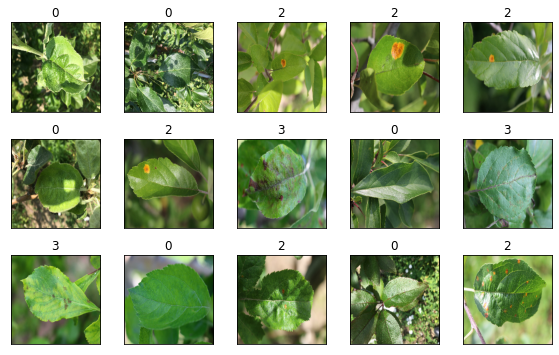
\includegraphics[width=800px,height=500]{Images/InputImages} 

}

\caption{**FIGURE 1.** Sample of training images.}\label{fig:input-images}
\end{figure}

Although we have ultimately decided not to apply the \textbf{PCA} to
reduce the dimensionality of the dataset, we believe it might be
interesting to visualize the first ten principal directions and
qualitatively compare them with a sequence of principal directions with
lower retained variance. As we can appreciate in the figures reported in
the \protect\hyperlink{pca}{Appendix}, the principal components with
lower retained variance correspond to almost pure noise and from the
retained variance assesment (using the criterion of 90\% variance
retention) we have obtained 429 components.

Here instead we visualize the first two principal components of a
\textbf{truncated SVD} to qualitatively investigate the linear
separability of the dataset \footnote{\textbf{Assumption}: if the
  dataset is linearly separable, the direction along which which the
  classes diverge is one of the principal components with larger
  retained variance, otherwise the noise would be greater than the
  signal.}.

\begin{figure}

{\centering 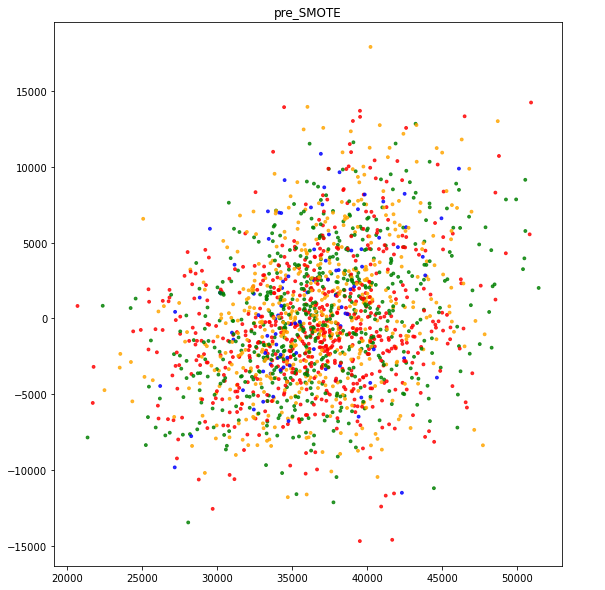
\includegraphics[width=450px,height=450]{Images/TruncatedSVD_preSMOTE} 

}

\caption{**FIGURE 2.** Pre-`SMOTE` truncated SVD.}\label{fig:pre-smote}
\end{figure}

As one could have resonably expected given such a high dimensionality,
the dataset is not linearly separable.

Later in the report we will describe an attempt using a
\protect\hyperlink{ae}{convolutional autoencoder}, while in the next
section we can verify the amplification of the classes performed by
\texttt{SMOTE} and recognize the clustering of the generated points.

\hypertarget{methodology}{%
\subsection{\texorpdfstring{\textbf{Methodology}}{Methodology}}\label{methodology}}

\hypertarget{smote}{%
\subsubsection{\texorpdfstring{Class Balancing with
\texttt{SMOTE}}{Class Balancing with SMOTE}}\label{smote}}

\texttt{SMOTE(sampling\_strategy,\ k\_neighbors)} is a class balancing
algorithm that operates as follows:

\begin{enumerate}
\def\labelenumi{\arabic{enumi}.}
\tightlist
\item
  (one of) the minority class(es) is considered ;
\item
  a point is randomly chosen and its first \texttt{n\_neighbors} nearest
  neighbors are found ;
\item
  one of those nearest neighbors is then randomly selected, and the
  vector between this point and the originally selected point is drawn ;
\item
  this vector is multiplied by a number between 0 and 1, and the
  resulting synthetic point is added to the dataset.
\end{enumerate}

Besides the baseline variant, \texttt{SVMSMOTE} and \texttt{ADASYN} have
been tested too:

\begin{itemize}
\tightlist
\item
  \texttt{SVMSMOTE} starts by fitting an SVM on the data, identifies the
  points which are more prone to mis-classification (i.e.~those on the
  border of the class cluster) via its support vectors and then will
  oversample those points more than the others.
\item
  \texttt{ADASYN} instead draws from a distribution over the minority
  class(es) that is pointwise inversely proportional to their density,
  so that more points are generated where the minority class(es) are
  sparser, and less points where they are more dense.
\end{itemize}

We have obtained the best performance applying baseline \texttt{SMOTE}
with some fine-tuning on the \texttt{sampling\_strategy} \footnote{The
  value \texttt{all} means that all classes are resampled to match the
  size of the majority class.} and the \texttt{n\_neighbors} parameters.
For more details see \protect\hyperlink{platform-limitations}{Platform
Limitations}.

\begin{figure}

{\centering 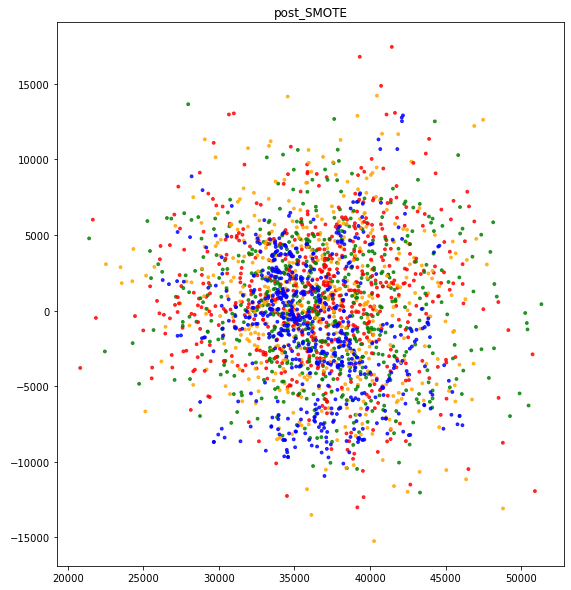
\includegraphics[width=450px,height=450]{Images/TruncatedSVD_postSMOTE} 

}

\caption{**FIGURE 3.** Post-`SMOTE` truncated SVD.}\label{fig:post-smote}
\end{figure}

\hypertarget{data-generator}{%
\subsubsection{\texorpdfstring{Data Augmentation with Keras
\texttt{ImageDataGenerator}}{Data Augmentation with Keras ImageDataGenerator}}\label{data-generator}}

We have adopted the Keras \texttt{ImageDataGenerator} and, after a
manual inspection of the images, we found that the best data
augmentation technique was a random planar rotation combined with random
horizontal flip. \footnote{For further information read the
  \href{https://keras.io/api/preprocessing/image/}{Keras image
  pre-processing API}.}

\hypertarget{exploration}{%
\subsubsection{Model Architecture Exploration}\label{exploration}}

We have implemented an extensive exploration of all models and here is
reported the \textbf{grid search} that achieved the best performance:

\begin{enumerate}
\def\labelenumi{\arabic{enumi}.}
\tightlist
\item
  some exploration and fine-tuning of the layers and parameters of the
  models (i.p. a dropout layer for the \texttt{EKM} only)
\item
  variations of the optimizer (for the \texttt{EKM} only)
\item
  optimal dropout and epoch number search
\item
  checkpointing
\end{enumerate}

We couldn't implement \textbf{early stopping} both in \texttt{EKM} and
\texttt{DenseNet121}, since the fluctuations in either validation loss,
categorical accuracy or mean column-wise ROC AUC where too high to
properly set the \texttt{min\_delta} and \texttt{patience} parameters in
the
\href{https://www.tensorflow.org/api_docs/python/tf/keras/callbacks/EarlyStopping}{TensorFlow
implementation}.

The best choice of the optimizer for the \texttt{EKM} proved to be the
\texttt{RMSprop}, while the standard \texttt{adam} performed pretty well
with the \texttt{DenseNet121}.

The manual implementations of the dropout and early stopping searches
acted simultaneoulsy, so they performed like a grid search.

The dropout, epoch values and weight corresponding to the highest mean
column-wise ROC AUC were saved and used during testing phase.

Later, in order to establish the quantitative impact of stocasticity in
weights initialization on the \texttt{EKM}, an EKM model with the best
drop is trained and validated, and the best epochs of this model and its
analogon trained and validated previously are compared: there was a
small difference, so we decided to make three submissions: one with the
baseline model re-trained on all data and with th best drop, one with a
model formed from the bst weights founfd before, and one with the
DenseNet.

Besides fluctuatios, we noticed that the DenseNet tends to occasionally
reach higher submission scores.

Considering the fact that optimal epoch number varies with trains et
size, a possible third attempt would have seen the best epoch number to
use in test phase, when the model is retrained on all train data,
extrapolated from a (best-epoch) vs (training set size) plot (given
stocasticity was not relevant), but this has unfortunately been
impossible due to two reasons: a techinical difficulty in combining
scikit's Leraning curves with a era smodel necessarily trained with
generators, and platform RAM limitations.

\hypertarget{ae}{%
\subsubsection{Convolutional Autoencoder}\label{ae}}

Putting a Covolutional Autoencoder between the Smoted \& augmented data
and the model training, despite the multiple configurations tried, the
best we could get is a \(0.7\) column-averaged ROC. The reason behind it
could be the fact that on one hand an autoencoder with no pooling on the
encoder side makes little sense in terms of dimensionality reductions,
while on the other hand even a single bidimensonal maxpooling caused the
output image to be too little for last EKM layer to classify. See
\protect\hyperlink{limitations}{Platform limitations} and see
\protect\hyperlink{model-architecture}{Model architecture} .

The only way way we managed to at least run it and see some loss drop
was to build a very shallow autoencoder (just a couple of layers besides
the input and the output), with the result that the loss didn't decrease
much. Anyway, inspired by the work of others and by some trial and
error, we had a chance to collect some architectural criteria to build
an convolutional autoencoder that at least learns. The folowing is to be
intended as an empirical recipe, with no or little theoretical
foundation of the reasons behind its ingredients. The autoencoder is
divided in an encoder and a decoder. The encoder should of course start
with an input layer, followed by some blocks of Conv2D and Pooling
layers (in our case it was MaxPooling2D). Deeper layers should have
decreasing filter numbers (for images as big as ours, a range from 64 to
32 should work). The decoder should start with a specular copy of the
encoder, where Conv2D layers are substituted by Conv2DTranspose,Pooling
by UpSampling. The decoder shall then have as its last two layers a
BatchNormalization layer and Conv2DTranspose with 3 filters (in order to
be able to compare output with input) activated by a sigmoid (this
explains the BatchNormalization layer). The unknown numner of
Conv2D-pooling blocks in the encoder (that determines the number of
Conv2DTranspose-UpSampling in the decoder) has to be jointly concocted
with the number of Conv2D-pooling layers of the network (see
\protect\hyperlink{model-architecture}{Model Architecture})

\begin{figure}

{\centering 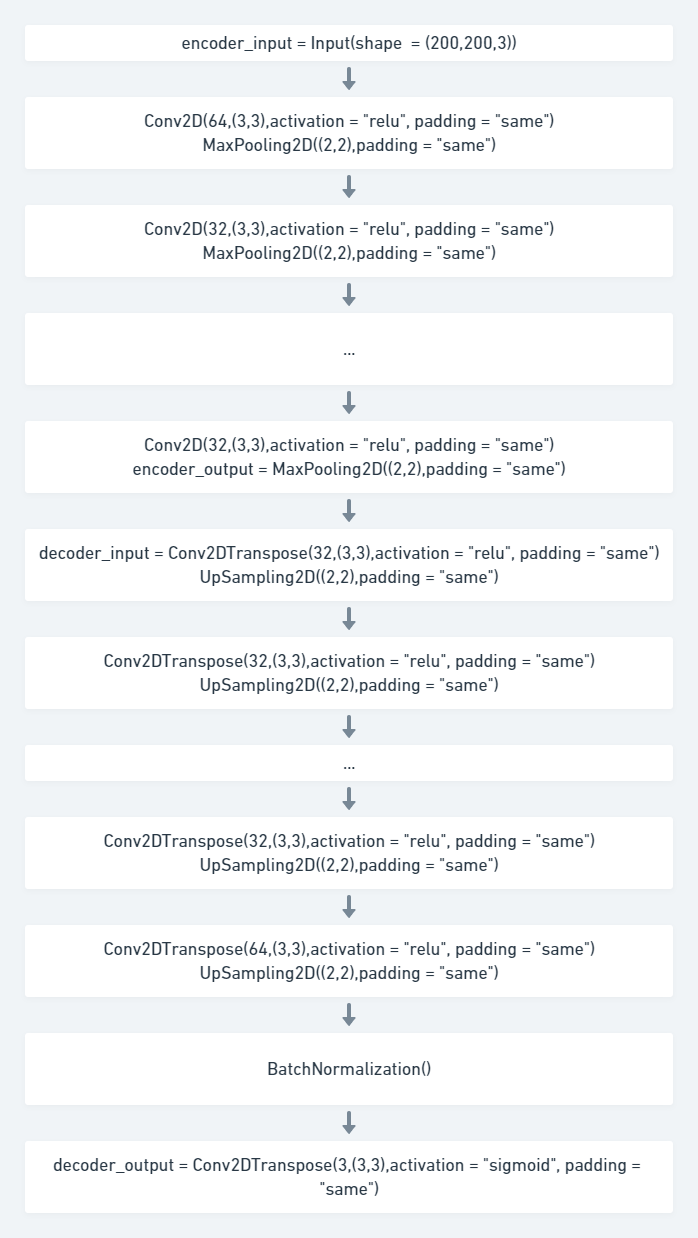
\includegraphics[width=350px,height=500]{Images/AEShort} 

}

\caption{**FIGURE 4.** Schematic representation of the convolutional autoencoder.}\label{fig:ae}
\end{figure}

\hypertarget{model-arcitecture}{%
\subsubsection{Selected Model Architecture}\label{model-arcitecture}}

Some online resaerch and trial and error with the network architecture
gave us some clues about how to build from scratch an effective, dataset
dependent model for image classifcation tasks. the network should of
course start with a Input layer, followed by blocks of Conv2D-Pooling
(MaxPooling in our case) layers. The number of these blocks should be
such that the last of them outputs a representation of \(n \times n\)
pixels ( \(\times c \, \,\) channels) where \(n\) is of the order of
units. This should be then followed by \(1-2\) dense layers, and a final
dense classifier layer. If The classification is binary (sigmoid), then
the last layer should be preceeded by a BatchNormlization layer.

\begin{figure}

{\centering 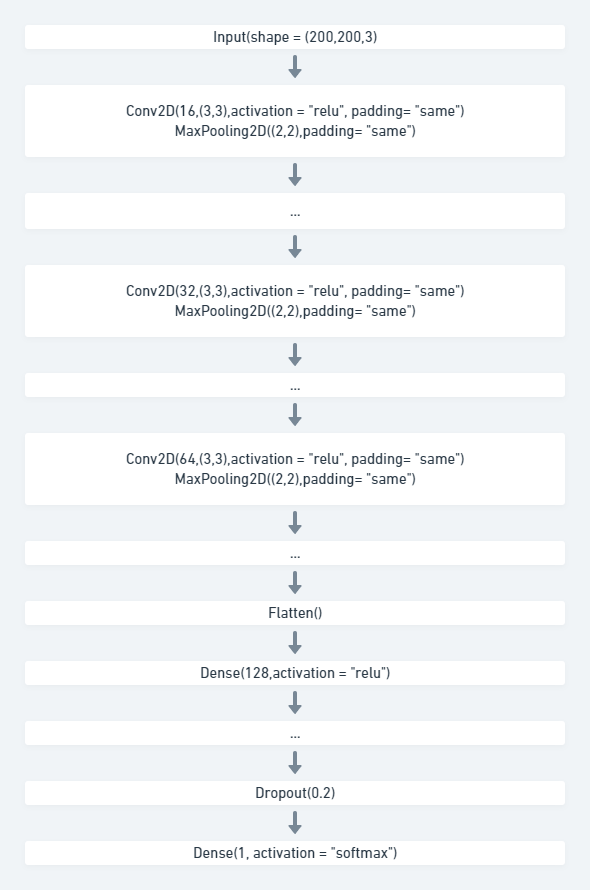
\includegraphics[width=350px,height=500]{Images/BaseNetShort} 

}

\caption{**FIGURE 5.** Schematic representation of the selected model architecture.}\label{fig:basenet}
\end{figure}

\hypertarget{results}{%
\subsection{\texorpdfstring{\textbf{Results}}{Results}}\label{results}}

The performance of the models has been evaluated on \textbf{mean
column-wise ROC AUC}: 0.972 for \texttt{DenseNet121} and 0.937 for
\texttt{EKM}.

\begin{figure}

{\centering \includegraphics[width=800px,height=550]{report_files/figure-latex/confusion-matrices-1} 

}

\caption{**FIGURE 6.** Confusion matrices of `EKM` (left) and `DenseNet121` (right).}\label{fig:confusion-matrices}
\end{figure}

\hypertarget{references}{%
\subsection{\texorpdfstring{\textbf{References}}{References}}\label{references}}

\begin{enumerate}
\def\labelenumi{\arabic{enumi}.}
\tightlist
\item
  \href{https://www.kaggle.com/c/plant-pathology-2020-fgvc7}{Plant
  Pathology 2020 - FGVC7: Identify the category of foliar diseases in
  apple trees}, \emph{Kaggle} (2020).
\item
  Ranjita Thapa et al. \href{https://arxiv.org/abs/2004.11958}{The Plant
  Pathology 2020 challenge dataset to classify foliar disease of
  apples}, \emph{arXiv pre-print} (2020).
\item
  Gao Huang et al. \href{https://arxiv.org/abs/1608.06993}{Densely
  Connected Convolutional Networks}, \emph{arXiv pre-print} (2018).
\end{enumerate}

\hypertarget{appendix}{%
\subsection{\texorpdfstring{\textbf{Appendix}}{Appendix}}\label{appendix}}

\hypertarget{additional-material}{%
\subsubsection{Related Material}\label{additional-material}}

\begin{itemize}
\tightlist
\item
  Explore the
  \href{https://github.com/InPhyT/NeuralNetworksProject}{GitHub
  repository} of the project.
\item
  Read the code in the
  \href{https://nbviewer.jupyter.org/github/InPhyT/NeuralNetworksProject/notebook.ipynb}{Jupyter
  notebook}.
\item
  Run the code in the
  \href{https://www.kaggle.com/inphyt2020/neuralnetworksproject}{Kaggle
  notebook}.
\end{itemize}

\hypertarget{platform-limitations}{%
\subsubsection{Platform Limitations}\label{platform-limitations}}

Since the last unstable version of GPU-supported TensorFlow is required
to run the code and we haven't been able to set the proper kernels up on
our local machines, we have been constrained to rely on a publicly
available cloud interactive environment like \emph{Kaggle}, which
provided free out of the box kernels for our purposes. The only
limitations are in terms of CPU RAM, which forced us to downsize the
images to about 200 \(\times\) 200 pixels.

\hypertarget{visualization}{%
\subsubsection{Visualization}\label{visualization}}

\hypertarget{pca}{%
\paragraph{\texorpdfstring{\emph{PCA}}{PCA}}\label{pca}}

\begin{figure}

{\centering 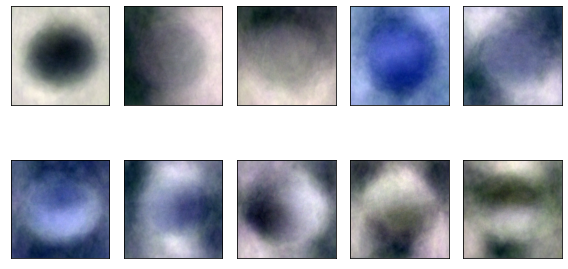
\includegraphics[width=800px,height=400]{Images/PCA1} 

}

\caption{**FIGURE 7.** The first ten principal directions of the PCA.}\label{fig:pca1}
\end{figure}
\begin{figure}

{\centering 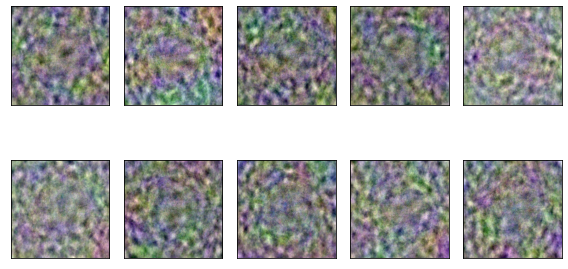
\includegraphics[width=800px,height=400]{Images/PCA200} 

}

\caption{**FIGURE 8.** Directions 200-210 of the PCA.}\label{fig:pca200}
\end{figure}
\begin{figure}

{\centering 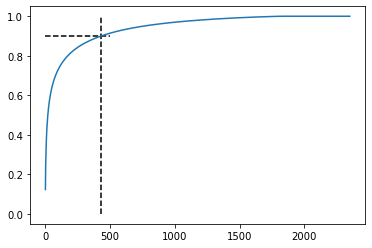
\includegraphics[width=550px,height=400]{Images/ExplainedVariance90} 

}

\caption{**FIGURE 9.** Explained Variance.}\label{fig:variance}
\end{figure}

\hypertarget{filters-featuremaps}{%
\paragraph{\texorpdfstring{\emph{Filters and Activation
Maps}}{Filters and Activation Maps}}\label{filters-featuremaps}}

\begin{figure}

{\centering 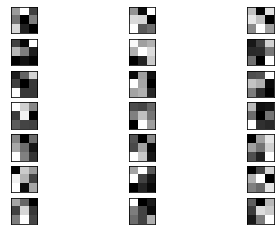
\includegraphics[width=550px,height=460]{Images/FiltersEKM} 

}

\caption{**FIGURE 10.** Three channels with some of the first 3x3 filters of the `EKM`.}\label{fig:filters-ekm}
\end{figure}

\begin{figure}

{\centering 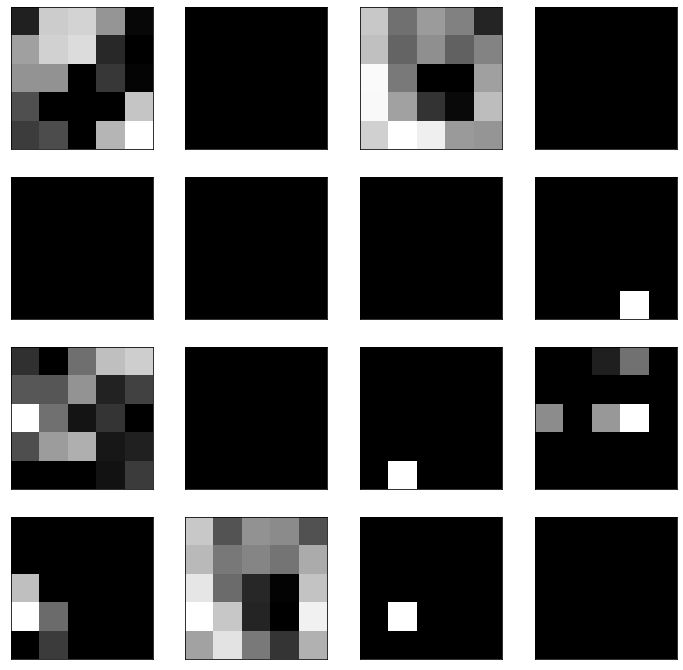
\includegraphics[width=9.5in]{Images/FeatureMaps2} 

}

\caption{**FIGURE 11.** Activation maps of the second hidden layer of `EKM`.}\label{fig:maps2}
\end{figure}
\begin{figure}

{\centering 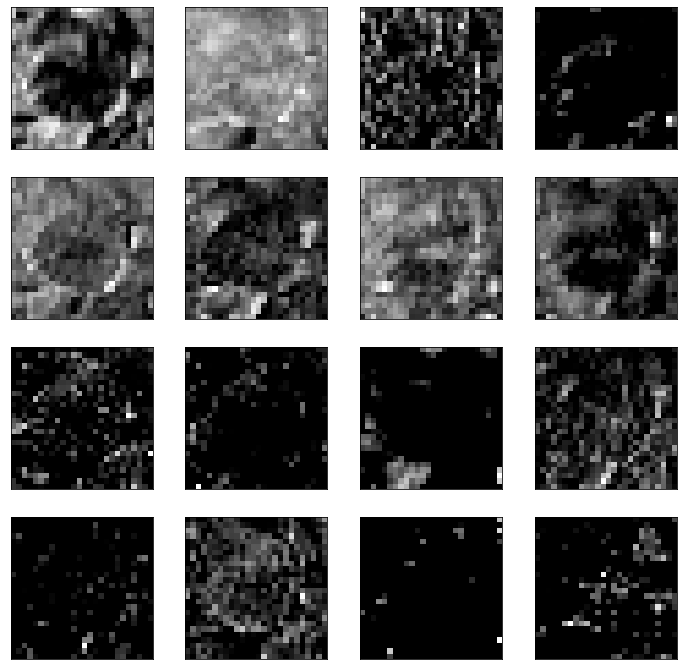
\includegraphics[width=9.5in]{Images/FeatureMaps6} 

}

\caption{**FIGURE 12.** Activation maps of the sixth hidden layer of `EKM`.}\label{fig:maps6}
\end{figure}
\begin{figure}

{\centering 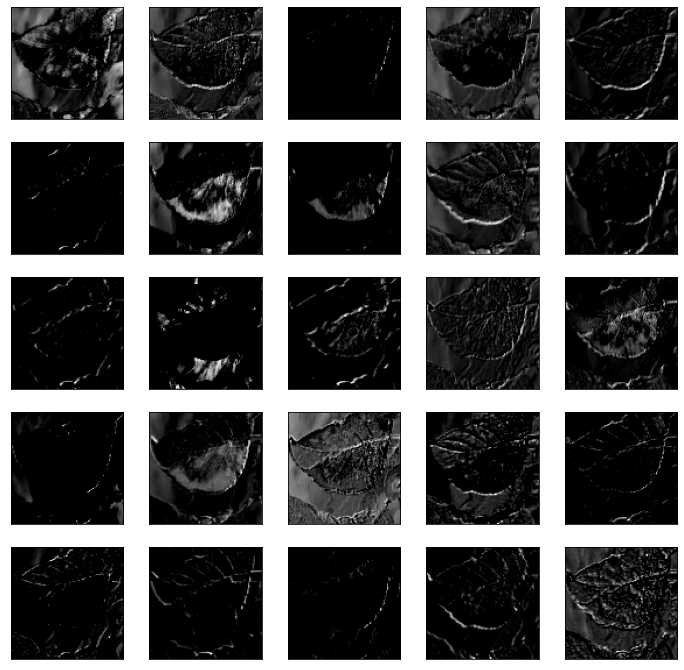
\includegraphics[width=9.5in]{Images/FeatureMaps9} 

}

\caption{**FIGURE 13.** Activation maps of the ninth hidden layer of `EKM`.}\label{fig:maps9}
\end{figure}

\end{document}
